\subsection{Modelos de Aprendizado de M\'aquina Supervisionados}\label{subsec:reg}

Os modelos regressivos para séries temporais têm sido amplamente reconhecidos e utilizados na literatura atual, especialmente aqueles baseados em métodos de gradiente. Esses modelos, incluindo a regressão linear simples, têm se destacado como uma escolha popular em competições de séries temporais em todo o mundo.

Esses modelos são valorizados por sua capacidade de capturar relações complexas e não lineares nos dados, permitindo previsões mais precisas e eficientes. Sua popularidade reflete o reconhecimento da eficácia desses modelos em abordar uma ampla gama de problemas de previsão de séries temporais em diferentes áreas de estudo.

A abordagem regressiva, combinada com técnicas de otimização baseadas em gradiente, tem se mostrado particularmente eficaz na obtenção de resultados de alta qualidade. Esses modelos são capazes de aprender a partir dos dados históricos e ajustar seus parâmetros de forma iterativa, otimizando assim o desempenho da previsão.

Com a crescente disponibilidade de dados e avanços na área de aprendizado de máquina, espera-se que os modelos regressivos para séries temporais continuem a evoluir e desempenhar um papel importante na análise e previsão de dados temporais em diversas aplicações.

\subsubsection{Regress\~ao Linear (LR)}

De acordo com o estudo realizado por \citeonline{korstanje2021}, nos modelos de aprendizado de máquina supervisionados, é feita uma tentativa de identificar as relações existentes entre diferentes variáveis:


\begin{itemize}
	\item Variável de destino: a variável que você tenta prever
	\item Variáveis explicativas: Variáveis que ajudam você a prever o alvo variável
\end{itemize}

Para realizar previsões, é importante que se compreenda quais tipos de variáveis explicativas podem ser utilizadas. Neste exemplo, a variável \textbf{Pressão de Sucção (PT01SU)} será considerada como a variável $x$, enquanto a variável \textbf{Nível do Reservatório (Câmara 1) LT01} será considerada como a variável $y$, com base na análise de correlação de Pearson ilustrada na Figura \ref{fig:person}. O coeficiente de correlação indica a relação entre o eixo $x$ e $y$, como expresso pela seguinte fórmula.



A fórmula do coeficiente de correlação de Pearson é dada por:

\begin{equation}
	r=\frac{\sum\left(x_i-\bar{x}\right)\left(y_i-\bar{y}\right)}{\sqrt{\left(\sum\left(x_i-\bar{x}\right)^2\right)\left(\sum\left(y_i-\bar{y}\right)^2\right)}}
\end{equation}

Onde $x_i$ e $y_i$ representam os valores das variáveis $X$ e $Y$, respectivamente. $\bar{x}$ e $\bar{y}$ são as médias dos valores $x_i$ e $y_i$. O coeficiente de correlação de Pearson mede a força e a direção da relação linear entre as variáveis $X$ e $Y$. Valores próximos a 1 indicam uma correlação positiva forte, valores próximos a -1 indicam uma correlação negativa forte, e valores próximos a 0 indicam uma ausência de correlação entre as variáveis.

\begin{figure}[H]
	\centering
	\caption{Corelação de Pearson}
	\label{fig:person}
	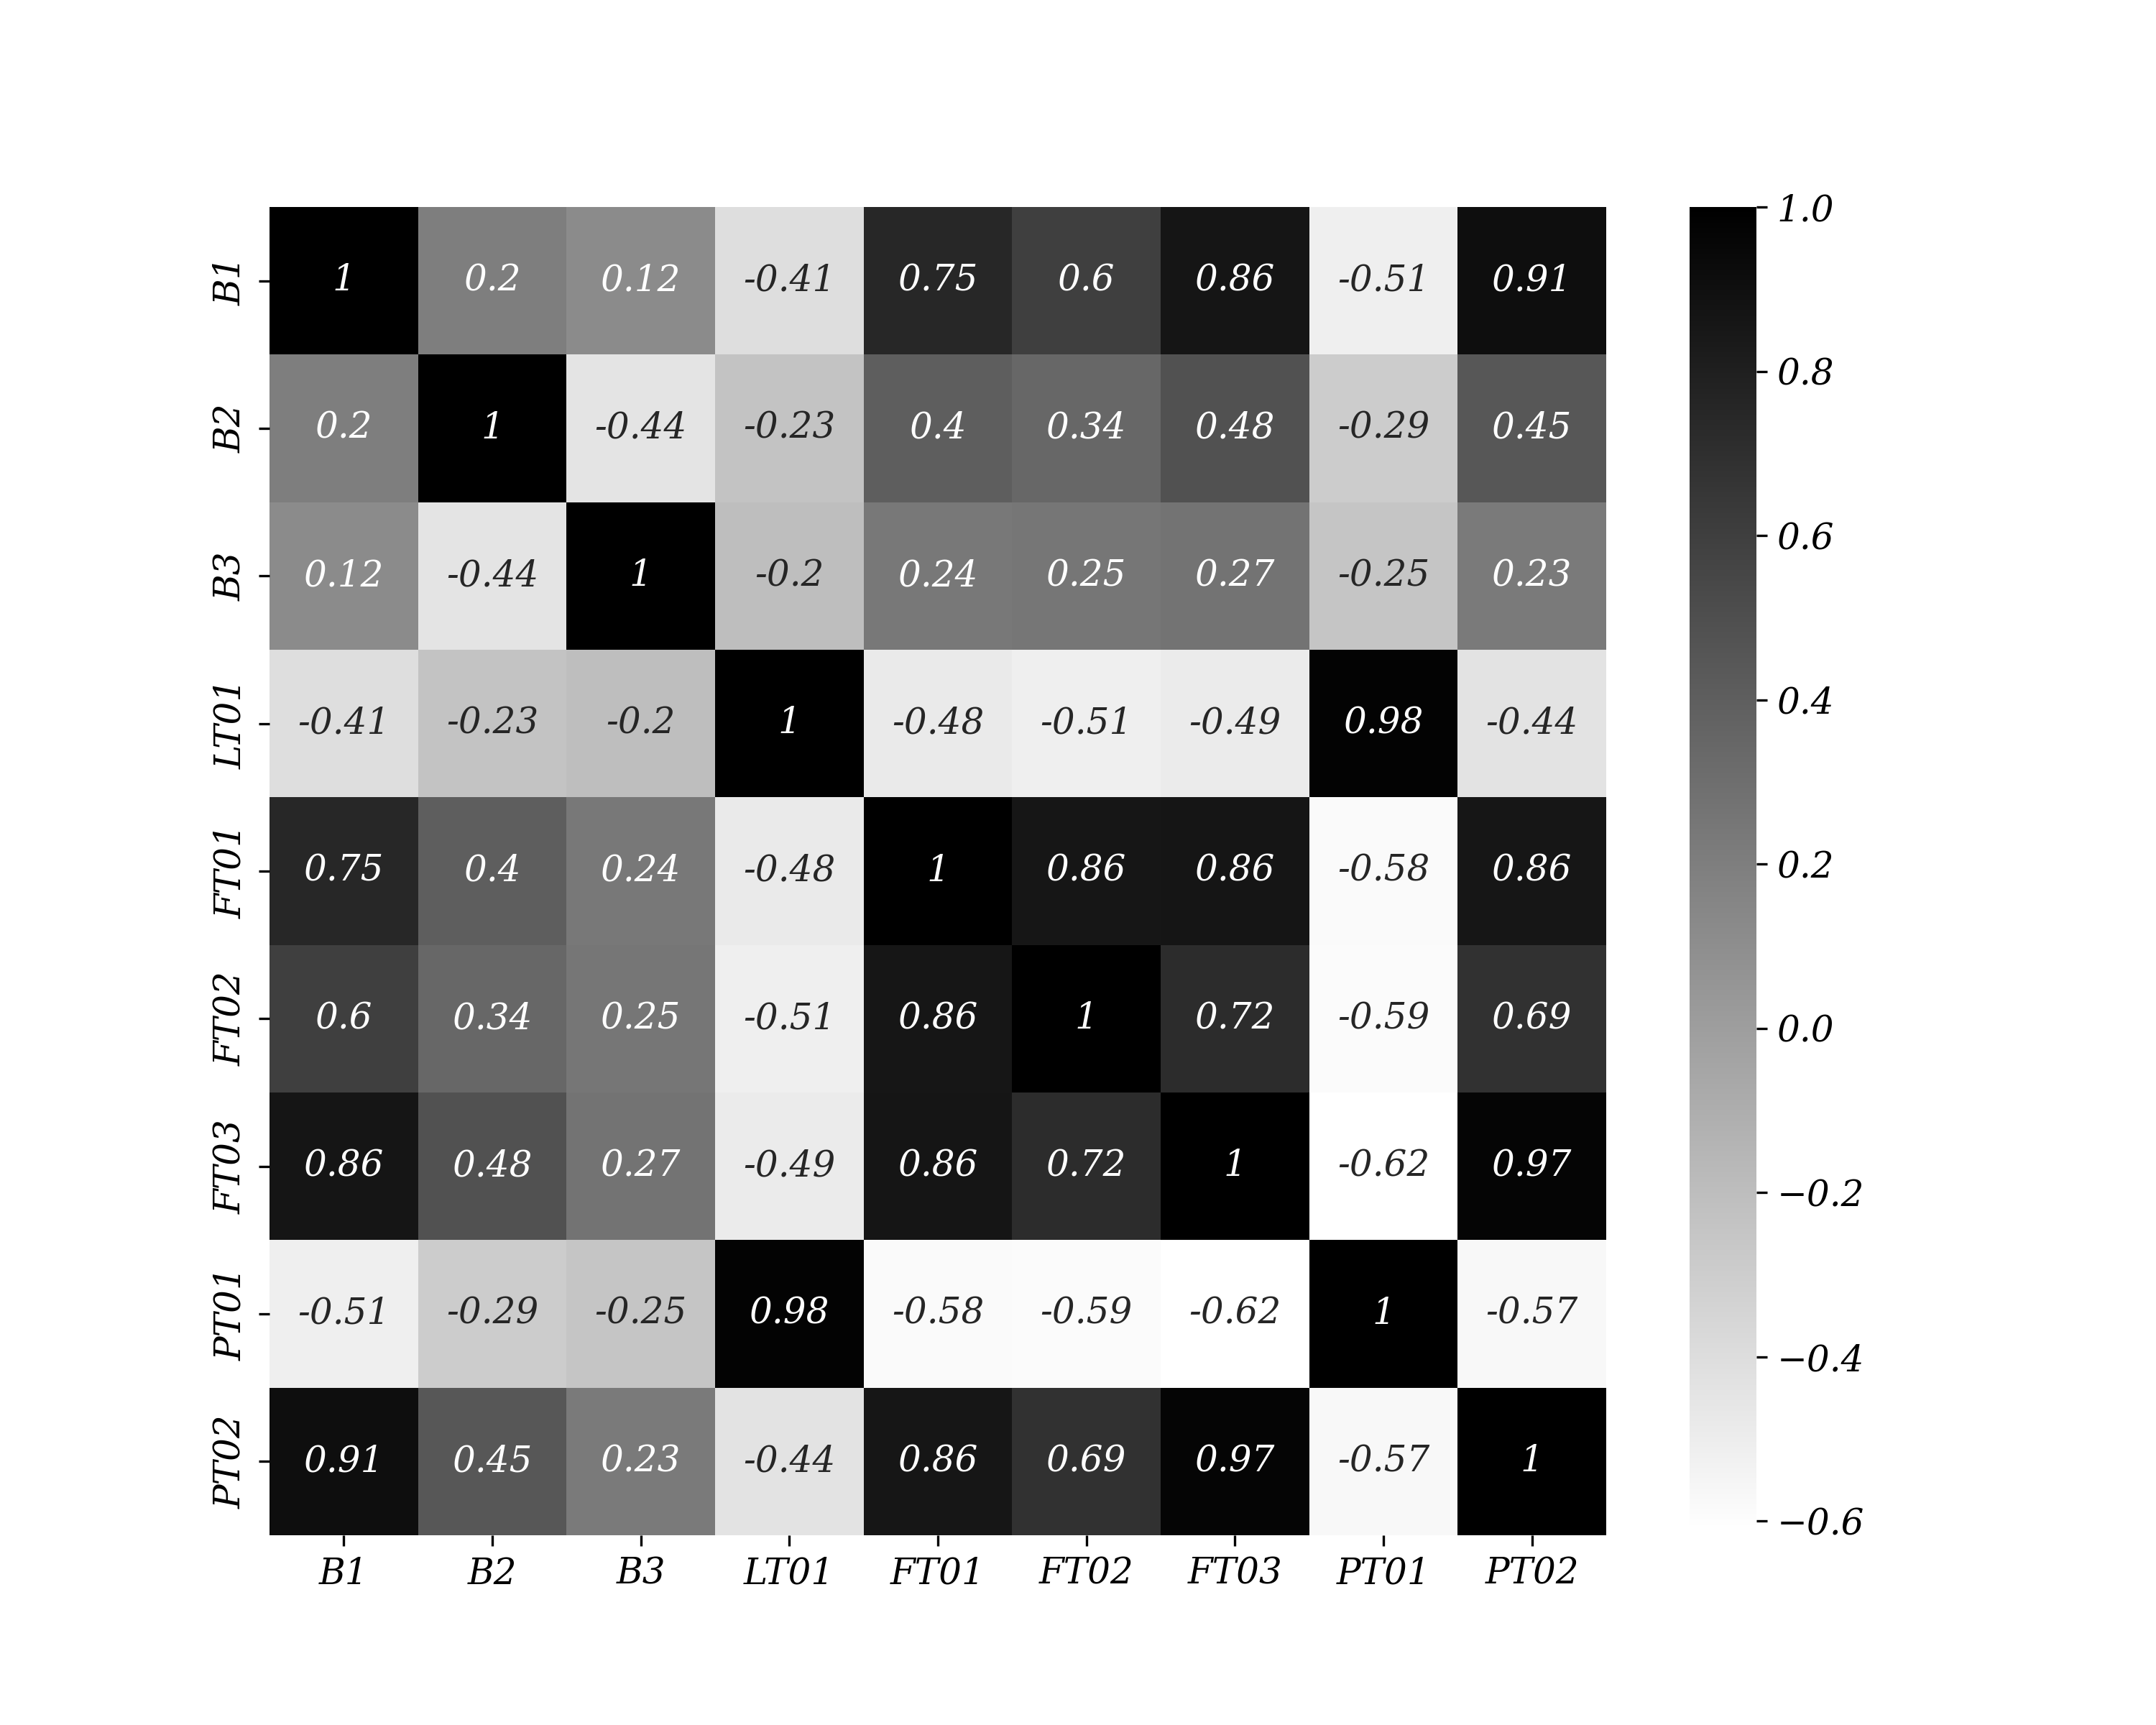
\includegraphics[width=1\linewidth]{Apendices/Figuras/modelagem-24h/person}
	
	\fonte{Elaboração própria a partir de dados da SANEPAR (2018 a 2020)}
\end{figure}

A Figura \ref{fig:person} ilustra a correlação entre as variáveis no conjunto de dados em questão. Essa imagem representa graficamente a relação entre as variáveis e é usada para demonstrar a existência de uma correlação forte entre elas. Com base nessa análise, é possível responder à pergunta de pesquisa \ref{q1}, pois a correlação entre as variáveis é significativa.

\subsubsection{Defini\c c\~ ao do modelo}

A regressão linear é definida da seguinte forma:

\begin{equation}
	y = \beta_0 + \beta_1 x_1 + \cdots + \beta_p x_p + \varepsilon \label{eq:lr}
\end{equation}

Da Equação \eqref{eq:lr}, temos as seguintes variáveis:

\begin{itemize}
	\item Há $p$ variáveis explicativas, denotadas por $x$.
	\item Existe uma variável alvo, denotada por $y$.
	\item O valor de $y$ é calculado como uma constante $\beta_0$, somada aos valores das variáveis $x$ multiplicados por seus coeficientes $\beta_1$ a $\beta_p$.
\end{itemize}

\begin{figure}[H]
	\centering
	\caption{Regressão linear LT01 vs PT01 correlação 98\%}
	\label{fig:lr-lt01-m3}
	\includegraphics[width=1\linewidth]{"Modelos/Figuras/LR LT01 (m³)"}
	
	\fonte{Elaboração própria a partir de dados da SANEPAR (2018 a 2020)}
\end{figure}



A Figura \ref{fig:lr-lt01-m3} fornece uma representação visual da interpretação dos coeficientes $\beta_0$ e $\beta_1$. Ela ilustra que um aumento de $1$ na variável $x$ está associado a um aumento proporcional de $\beta_1$ na variável $y$. O valor de $\beta_0$ representa o valor de $y$ quando $x$ é igual a $0$.

Para utilizar a regressão linear, é necessário estimar os coeficientes (betas) com base em um conjunto de dados de treinamento. Esses coeficientes podem ser estimados por meio da seguinte fórmula, expressa em notação matricial:

\begin{eqnarray}
	\hat{\beta}&=&\left(X^T X\right)^{-1} X^T y\label{eq:ols}
\end{eqnarray}

A fórmula mencionada, conhecida como \textbf{OLS} (método dos mínimos quadrados ordinários), é amplamente utilizada na regressão linear \citeonline{korstanje2021}. Esse método é conhecido por ser rápido de ajustar, pois requer apenas cálculos matriciais para estimar os coeficientes $\beta$. No entanto, ele é mais adequado para processos lineares e pode ser menos adequado para modelos mais complexos que envolvam relações não-lineares. Portanto, é importante considerar suas limitações ao aplicar a regressão linear em contextos mais complexos.

\begin{figure}[H]
	\centering
	\caption{Regressão linear (LR) um passo a frente}
	\label{fig:1-regressao-linear}
	\includegraphics[width=1\linewidth]{Modelos/Figuras/regressão-linear}
	
	\fonte{Elaboração própria a partir de dados da SANEPAR (2018 a 2020)}
\end{figure}


\subsubsection{Floresta Aleat\'oria (Random Forest)} \label{subsubsec:rf}

Pode-se observar que ter exatamente a mesma árvore de decisão repetidas vezes não adiciona valor significativo em comparação a usar essa mesma árvore de decisão apenas uma vez. Em modelos de conjunto, cada modelo individual deve ser ligeiramente diferente dos demais. Existem dois métodos amplamente reconhecidos para criar conjuntos: o ensacamento (\textit{bagging}) e o reforço (\textit{boosting}). A floresta aleatória utiliza o ensacamento para criar um conjunto de árvores de decisão, onde cada árvore é construída com uma amostra aleatória do conjunto de dados original. Isso garante que as árvores sejam distintas e diversificadas, contribuindo para a robustez e eficácia do modelo.


\begin{figure}[H]
	\centering
	\caption{Regressão da Floresta Aleatória (RFR)}
	\label{fig:1-regressao-rfa}
	\includegraphics[width=1\linewidth]{Modelos/Figuras/regressão-rfa}
	
	\fonte{Elaboração própria a partir de dados da SANEPAR (2018 a 2020)}
\end{figure}


Segundo \citeonline{Pelletier2016156}, cada árvore em um modelo de Floresta Aleatória de Regressão (RFR) é construída por meio de um algoritmo de aprendizado individual que divide o conjunto de variáveis de entrada em subconjuntos, com base em um teste de valor de atributo, como o coeficiente de Gini. Ao contrário das árvores de decisão clássicas, as árvores de RFR são construídas sem poda e selecionam aleatoriamente um subconjunto de variáveis de entrada em cada nó. Atualmente, o número de variáveis utilizadas para dividir um nó em uma RFR (denotado por $m$) corresponde à raiz quadrada do número total de variáveis de entrada. Essa abordagem ajuda a aumentar a diversidade das árvores e aprimorar o desempenho do modelo.

\begin{figure}[H]
	\centering
	\caption{Esquema da Floresta Aleatória}
	\label{fig:rf}
	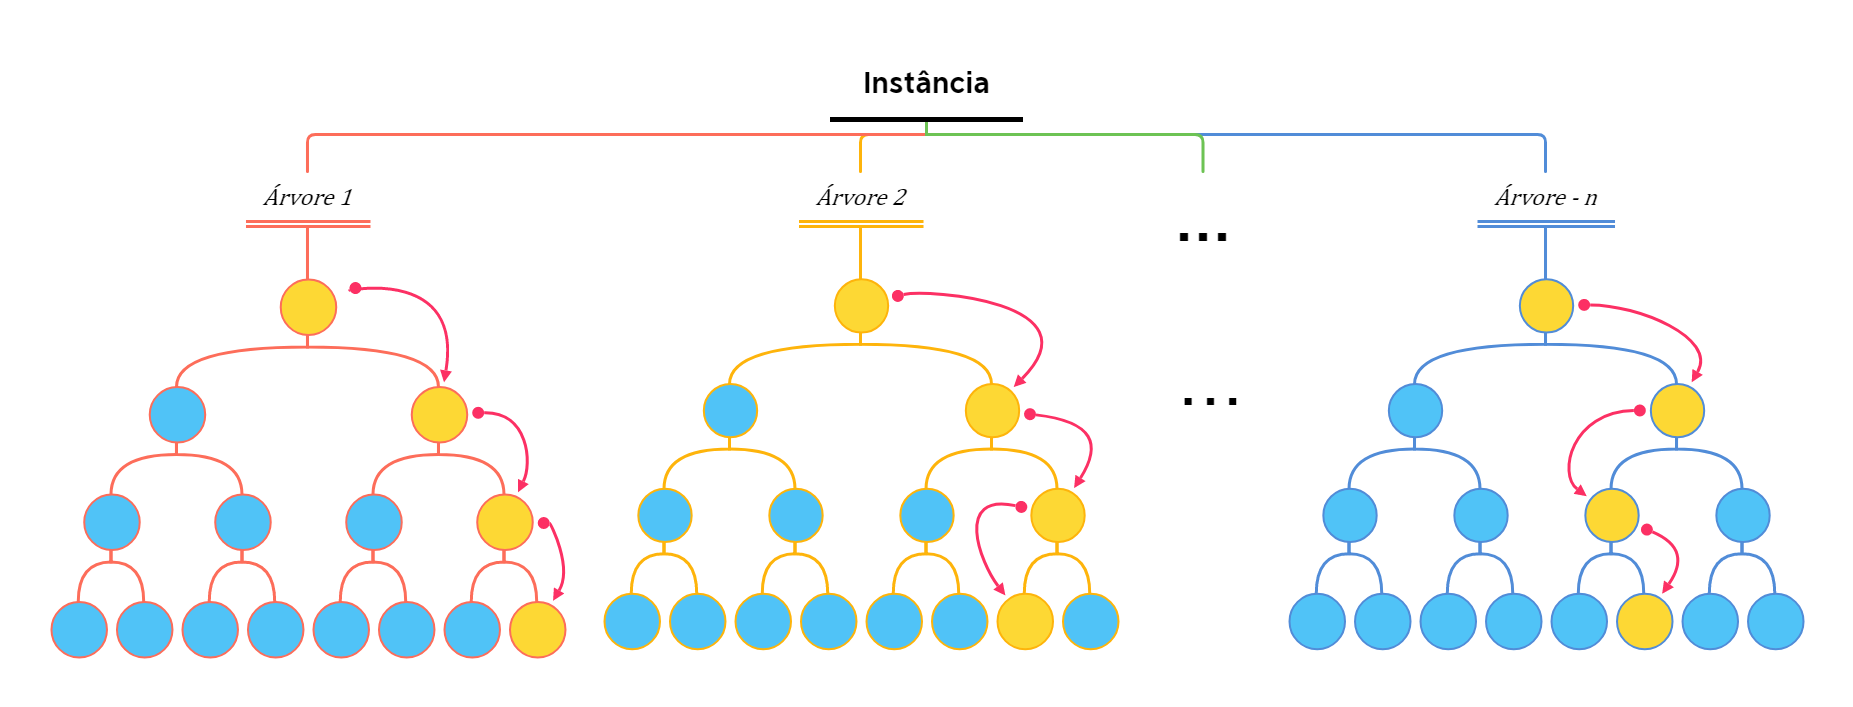
\includegraphics[width=1\linewidth]{Modelos/Figuras/RF}
	
	\fonte{Elaboração própria}
\end{figure}


\subsubsection{Gradient Boosting (como XGBoost, LightGBM)}\label{subsubsec:lgbxgb}

O aumento de gradiente (do inglês\textit{gradient boosting}) é um método que combina vários modelos de árvore de decisão para realizar previsões. Cada uma dessas árvores de decisão é única, pois a diversidade é um elemento importante nesse processo. A diversidade é alcançada através de um processo chamado boosting, que é uma abordagem iterativa. O boosting adiciona modelos fracos ao conjunto de forma inteligente, dando mais peso aos pontos de dados que ainda não foram bem previstos. 

O processo de boosting melhora o conjunto ao focar nas partes dos dados que ainda não são compreendidas. A Figura \ref{fig:xgboost} apresenta uma visão esquemática desse processo. À medida que novos modelos fracos são adicionados, todos os modelos fracos intermediários são mantidos. O modelo final é uma combinação de todos esses modelos fracos, resultando em um ensemble que oferece uma melhor capacidade de previsão do que um único modelo.

O boosting é apenas um dos métodos de ensemble utilizados em conjunto com o bagging. O bagging também é um método que utiliza múltiplos modelos de árvore de decisão, porém, em vez de adicionar os modelos de forma iterativa, cada modelo é treinado independentemente em subconjuntos aleatórios dos dados de treinamento. Ambos os métodos, boosting e bagging, têm como objetivo melhorar o desempenho do modelo combinando as previsões de múltiplos modelos individuais.


\begin{figure}[H]
	\centering
	\caption{Impulsionando gradiente com XGBoost e LightGBM}
	\label{fig:xgboos}
	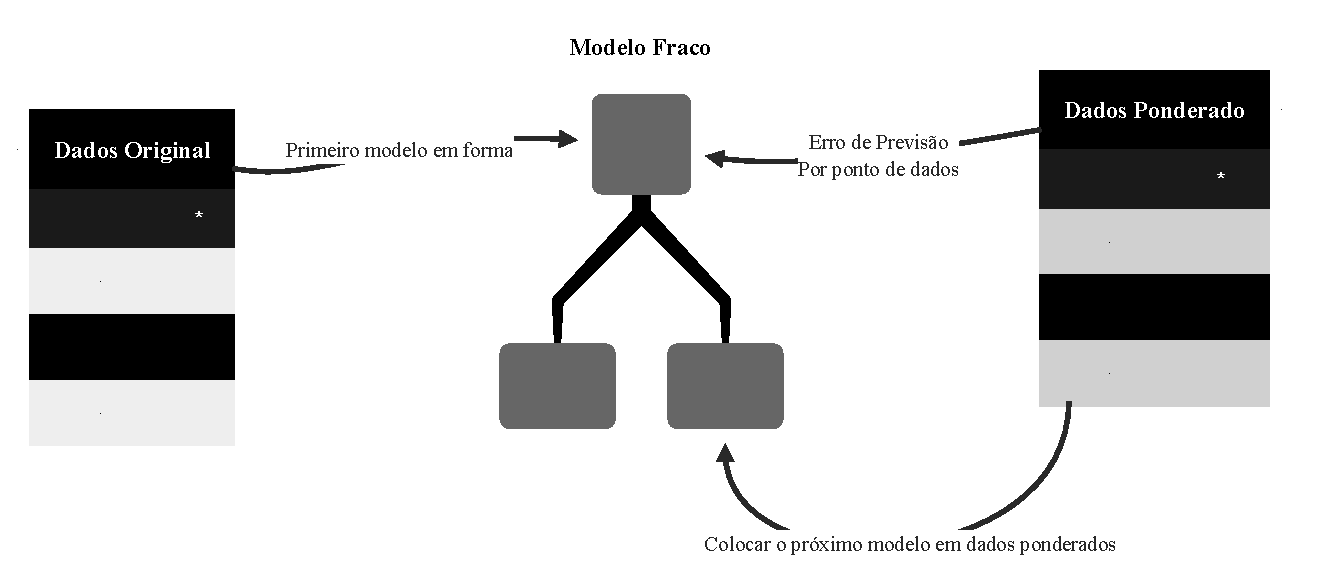
\includegraphics[width=1\linewidth]{Modelos/Figuras/xgboos}
	
	\fonte{Adaptação de \citeonline{korstanje2021}}
\end{figure}



\subsubsection{O Gradiente em Gradiente de Boosting (Refor\c co)} \label{subsubsec:boosting}

O processo iterativo utilizado no aumento de gradiente, como descrito por \citeonline{korstanje2021}, recebe esse nome por um motivo. O termo ``gradiente'' refere-se a um campo vetorial de derivadas parciais que apontam na direção da inclinação mais acentuada. De forma simplificada, podemos pensar nos gradientes como as inclinações das estradas: quanto maior a inclinação, mais íngreme a colina. Para calcular os gradientes, são realizadas derivadas ou derivadas parciais de uma função.

No aumento de gradiente, ao adicionar árvores adicionais ao modelo, o objetivo é incorporar uma árvore que explique melhor a variação que ainda não foi explicada pelas árvores anteriores. Dessa forma, a nova árvore tem como objetivo ajustar-se aos erros ou resíduos deixados pelas árvores anteriores.

\begin{equation}
	y-\hat{y} \label{eq:xb}
\end{equation}

A equação \eqref{eq:xb} pode ser reescrita como a derivada parcial negativa da função de perda em relação às previsões $\hat{y}$:

\begin{equation}
	y-\hat{y} = -\frac{\partial L}{\partial \hat{y}} \label{eq:xb2}
\end{equation}

Isso é definido como o objetivo da nova árvore a ser adicionada no modelo de aumento de gradiente, garantindo que ela explique a máxima quantidade de variação adicional no modelo geral. Essa é a razão pela qual o modelo é chamado de "aumento de gradiente" (``\textit{gradient boosting}'', em inglês). O processo utiliza o gradiente da função de perda para guiar a adição de novas árvores, buscando minimizar o erro e melhorar a capacidade do modelo em explicar a variação nos dados.

\subsubsection{Algoritmos de boosting de gradiente}

Existem muitos algoritmos que executam versões ligeiramente diferentes de aumento de gradiente. Quando o método de aumento de gradiente foi inventado, o algoritmo não tinha um desempenho tão bom, mas isso mudou com o advento do algoritmo AdaBoost: o primeiro algoritmo capaz de se adaptar a modelos fracos.

O algoritmo de aumento de gradiente é uma das ferramentas de aprendizado de máquina com melhor desempenho no mercado. Após o AdaBoost, uma longa lista de algoritmos de aumento levemente diferentes foi adicionada à literatura, incluindo XGBoost, LightGBM, LPBoost, BrownBoost, MadaBoost, LogitBoost e TotalBoost. Ainda há muitas contribuições para melhorar a teoria do aumento de gradiente. Nesta subseção, dois algoritmos são apresentados: XGBoost e LightGBM.

O \textbf{XGBoost} é um dos algoritmos de aprendizado de máquina mais utilizados. É uma forma rápida de obter bom desempenho. Devido à sua facilidade de uso e alto desempenho, é frequentemente o primeiro algoritmo escolhido por muitos profissionais de aprendizado de máquina.

O \textbf{LightGBM} é outro algoritmo de aumento de gradiente que é importante conhecer. Atualmente, é um pouco menos difundido que o XGBoost, mas está ganhando popularidade rapidamente. A vantagem esperada do LightGBM em relação ao XGBoost é um ganho de velocidade e uma utilização mais eficiente de memória.

Nesta subseção, você encontrará as implementações de ambos os algoritmos de aumento de gradiente.

\subsubsection{A diferen\c ca entre XGBoost e LightGBM}

Se alguém planeja utilizar os dois algoritmos de aumento de gradiente, é importante que essa pessoa compreenda suas diferenças, o que também proporciona uma visão das várias divergências que existem entre os modelos disponíveis no mercado.

Uma diferença fundamental reside na maneira como esses algoritmos identificam as melhores divisões entre os nós das árvores de decisão individuais. É crucial lembrar que uma divisão em uma árvore de decisão ocorre quando a árvore precisa encontrar a separação que mais melhora o desempenho do modelo.

A abordagem intuitiva e simples para encontrar a melhor divisão é iterar por todas as possibilidades e selecionar a melhor. No entanto, essa abordagem é computacionalmente custosa, e algoritmos mais recentes apresentam alternativas mais eficientes.

Uma alternativa proposta pelo XGBoost é a segmentação baseada em histograma. Nesse caso, em vez de iterar por todas as partições possíveis, o modelo constrói um histograma para cada variável e utiliza-os para encontrar a melhor divisão geral entre as variáveis.

O LightGBM, desenvolvido pela Microsoft, adota uma abordagem mais eficiente para a definição das divisões. Essa abordagem é conhecida como amostragem unilateral baseada em gradiente (GOSS). O GOSS calcula o gradiente para cada ponto de dados e utiliza-o para filtrar os pontos de dados com gradientes baixos. Afinal, os pontos de dados com gradientes baixos já são bem compreendidos, enquanto aqueles com gradientes altos precisam ser melhor aprendidos.

O LightGBM também utiliza uma abordagem chamada Exclusive Feature Bundling (EFB), que acelera a seleção de muitas variáveis correlacionadas. Outra diferença é que o modelo LightGBM é adequado para o crescimento de folhas (leaf-wise growth), enquanto o XGBoost cultiva as árvores em níveis (level-wise growth). Essa diferença pode ser visualizada na Figura \ref{fig:xgboost}.

Essa diferença teoricamente favorece o LightGBM em termos de precisão, mas também apresenta um maior risco de overfitting (sobreajuste) quando há poucos dados disponíveis. Portanto, é importante que a pessoa considere essas distinções ao escolher entre os dois algoritmos de aumento de gradiente.

\begin{figure}[H]
	\centering
	\caption{Compara-se o crescimento em folha com o crescimento em nível}
	\label{fig:xgboost}
	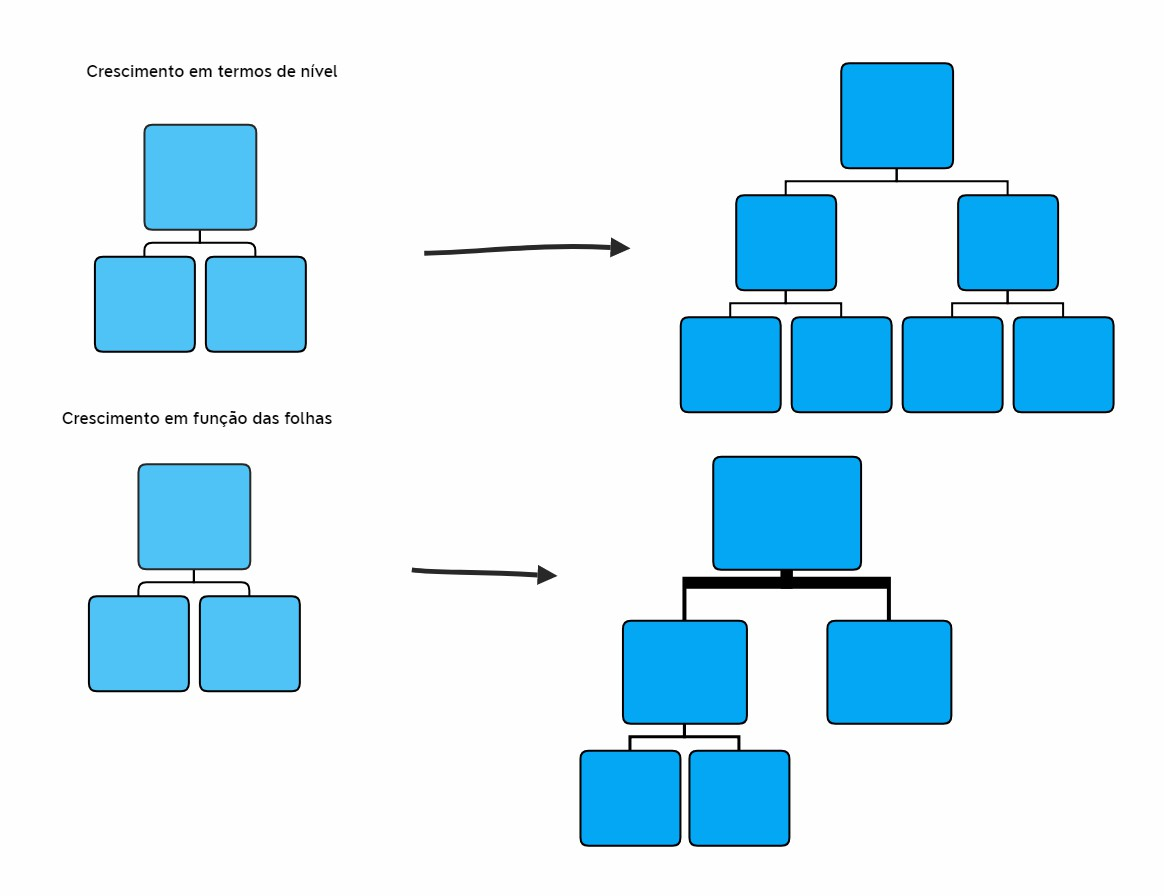
\includegraphics[width=1\linewidth]{Modelos/Figuras/xgboost}
	
	\fonte{Adaptação de \citeonline{korstanje2021}}
\end{figure}


Na Figura \ref{fig:xgboost}, é possível visualizar como cada modelo é ajustado durante o processo de crescimento de árvore em folhas e em níveis. Essa representação gráfica oferece uma compreensão visual das diferenças entre os dois métodos.

No crescimento de árvore em folhas, como no LightGBM, novas folhas são adicionadas à árvore de forma iterativa, visando maximizar a redução do erro de treinamento. Isso significa que as árvores são expandidas adicionando folhas, uma a uma, até que o critério de parada seja alcançado.

Por outro lado, no crescimento em níveis, como no XGBoost, as árvores são expandidas em profundidade de forma simultânea em todos os níveis. Ou seja, em cada nível, todas as folhas são expandidas ao mesmo tempo, resultando em um crescimento mais uniforme da árvore.

Essa distinção no modo de crescimento das árvores pode afetar o comportamento e o desempenho do modelo. Portanto, compreender essa diferença é importante ao escolher entre esses algoritmos de aumento de gradiente.

\begin{figure}[H]
	\centering
	\caption{A performance da regressão utilizando XGBoost e LightGBM é comparada}
	\label{fig:1-xgb-regressao}
	
	\begin{subfigure}{1\textwidth}
		\includegraphics[width=\linewidth]{Modelos/Figuras/xgb-regressão}
		\caption{Regressão XGBoost}	
	\end{subfigure}\hfill
	\begin{subfigure}{1\textwidth}
		\includegraphics[width=\linewidth]{Modelos/Figuras/lgbm-regressão}
		\caption{Regressão LightGBM}	
	\end{subfigure}
	
	\fonte{Elaboração própria a partir de dados da SANEPAR (2018 a 2020)}

\end{figure}	


Na Figura \ref{fig:1-xgb-regressao} é um modelo baseado nos dados coletados da SANEPAR.

